
\section{Implementation}

With a high level design in mind, we now discuss the implementation details.
We started by forking Linux from the GitHub {\tt git} mirror repository and
worked on x86\_64 Linux 3.0. We developed and tested incrementally on an 8-core
machine with 8BG of RAM running Arch Linux.

This section is divided into two logical parts. We first discuss the kernel
implementation, then the user library and in memory file system.

The first step was adding the three new syscalls: {\tt dput()}, {\tt dget()},
and {\tt dret()}. Our initial focus was adding process management related
functionality, then we added the {\tt Zero}, {\tt Copy}, and
{\tt Snapshot/Merge} operations in that order.

\subsection{Process synchronization}

The first step was adding the three new syscalls: {\tt dput()}, {\tt dget()},
and {\tt dret()}. Our initial focus was process creation and related
functionality. {\tt dput()} relies heavily on existing {\tt do\_fork()} and
{\tt do\_exit()} kernel code.
We added logic to enforce the requirement that deterministic processes cannot
outlive their parents. We blocked all external signals generated by user
applications, but allowed kernel-generated signals. We used the kernel-generated
signal mechanism to trigger implicit {\tt dret()}s on process faults like
divide-by-zero ({\tt SIGFPE}) and memory access violations ({\tt SIGSEVG}).

We augmented Linux's {\tt task\_struct} process structure with a new
\emph{deterministic PID} and low-level synchronization primitives. {\tt dput()}
and {\tt dget()} use these synchronization primitives to synchronize using the
fork-join model. When a parent starts a child
with {\tt dput()}, any subsequent {\tt dput()} or {\tt dget()} call blocks until
the child issues a {\tt dret()}.

Even though master processes have direct access to kernel I/O devices, we placed
some restrictions on what a master process can do. Processes
become the master of a deterministic process group by invoking {\tt dput()} with
a special parameter. The kernel makes sure that the process is not the parent of
any other nondeterministic process and isn't using any
unsupported virtual memory features, like ``kernel samepage
merging''~\cite{arcangeli2009increasing} or huge pages. Once a process
becomes a master, it can no longer use the legacy {\tt fork()} family of
syscalls. It can only create new processes through the deterministic family
of syscalls.

\iffalse
In Determinator, \emph{all} processes that issue a {\tt dput()} or {\tt dget()}
block until the child in question issues a {\tt dret()}. This is a limitation
for applications that benefit from concurrency, like running
{\tt make -j2}~\cite{Aviram10}. Determinator might miss opportunities to start
a parallel job, because a deterministic {\tt make} in Determinator schedules
itself and might be blocked waiting for a thread to finish when other children
are runnable. In our implementation we allow the master
process to perform a special non-blocking {\tt dget()} to determine whether or
not a child is still running. This allows more optimal scheduling, since the
root can find a runnable thread and give it work. Determinism is achieved by
recording the scheduling sequence for replay, if desired. This feature is
desirable for inherently nondeterministic applications like web servers that may
wish to exploit as much concurrency as possible.
\fi

\iffalse
\begin{itemize}
	\item Add three new syscalls with basic process creation, synchronization,
		and deletion.
	\begin{itemize}
		\item dput() relies heavily on existing fork() code to generate new processes.
		\item Disallow deterministic process reparenting: a deterministic or root
			process's death implies all children should die as well.
		\item Use existing code for handling process deletion: do\_exit().
		\item Block signals from reaching deterministic processes.
		\item Exceptions (e.g. divide-by-zero) immediately stop the process; parents
			must acknowledge and handle the child's exception.
	\end{itemize}
	\item Loosened root process requirements.
	\begin{itemize}
		\item The root process has the the option of being interrupted by a signal
			while waiting for a child via dput()/dget().
		\item Root processes may poll a children's runnability status to optimize
			scheduling of threads. This introduces non-determinism only for the root
			process which itself already has elevated permissions, but the scheduling
			sequence is still controllable and can be logged for debug replay.
\fi

Master processes can use {\tt dput()} to specify a set of signals to ignore
while in a blocking {\tt dput()} or {\tt dget()} (i.e. waiting for a child to
stop). This can be useful when a console operation wishes to
kill an application with a {\tt SIGINT}, but does not want other signals to
interrupt the master process.

The last feature relating strictly to process organization is register state
copying. The initial {\tt dput()} call that creates a child automatically
copies register state, since we effectively delegate work to {\tt fork()}.
Subsequent calls to {\tt dput()} and {\tt dget()} can put or retrieve a child's
general-purpose register state.

\iffalse
	\end{itemize}
	\item When dput() creates a child, it automatically copies the parent's
		register set into the child. Subsequent dput() calls can set/get a
		child's register state.
\fi

\subsection{Memory operations}

\label{sec:memop}

As mentioned in the section \ref{sec:challenges}, Linux's memory subsystem is
very complex. Before discussing how we implemented the memory operations,
we will give some technical background on Linux's memory subsystem. Our
implementation reused many existing functions, so this discussion will be
useful.

\begin{figure}
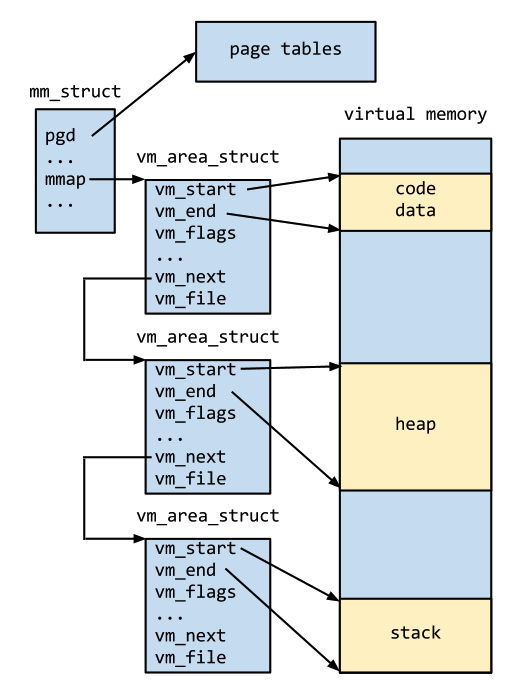
\includegraphics[scale=.42]{mm_struct.png}
\caption{Illustration of Linux's memory management data structures.}
\label{fig:mmstruct}
\end{figure}

\paragraph{Background}
A process's entire virtual memory is managed by a {\tt mm\_struct}.
{\tt mm\_struct}s maintain a list of contiguously mapped memory regions with
identical permission bits (e.g. read/write/execute); these regions are stored as
{\tt vm\_area\_struct}s (see Figure \ref{fig:mmstruct}). Anonymous memory
(memory not backed by a file) is mapped to a
read only global zero page, and new pages
are allocated \emph{on demand}~\cite{li1989memory}. In order to swap a single
physical page of memory to disk, Linux requires all mappings of the page have
the same offset from the start of the enclosing {\tt vm\_area\_struct} (see
Figure \ref{fig:anon_vma}). This
requirement makes swapping space and time efficient, but it places unfortunate
restrictions on how aggressively we can apply copy-on-write.

Linux provides {\tt dup\_mm()} to copy the virtual memory image of a process.
{\tt fork()} uses this to copy a process's memory via copy-on-write.
{\tt dup\_mm()} copies each {\tt vm\_area\_struct} of the source by invoking
{\tt copy\_page\_range()}. This function walks Linux's four level
page table structure to perform copy-on-write by actually changing page table
entries and marking the pages as read only.

Linux's memory subsystem does lack one important generality that is essential to
the core of Determinator's memory operations: in Linux, most virtual memory
kernel functions act on behalf
of the calling process (inside a syscall, the calling process is accessed via
the C macro {\tt current}) instead of operating on \emph{any} process's
virtual memory. For example, {\tt do\_mmap()}, which maps files into memory and
creates anonymous memory regions, will only perform work on {\tt current}.

\iffalse
	\item Memory operations are more difficult. Linux's memory subsystem is not
		as generic as I would have liked.
	\begin{itemize}
		\item The kernel supports zeroing an area of virtual memory, but only for
			the current running process that invoked a syscall. Most functionality
			in the memory subsystem works this way and is hardcoded this way.
		\item Before any real work could be done, I generalized some memory functions
			to work on any process (e.g. mmap\_region(), make\_pages\_present()).
		\item The copy\_page\_range() function copies a range of memory via
			copy-on-write, but it is really a helper function for fork() and is
			not very generic.
		\item copy\_page\_range() copies identical virtual memory regions.
		\item I wanted to support copy-on-write with an address offset, so I
			replicated copy\_page\_range()'s page table traversal code to allow
			the destination memory region to be offset by a page aligned amount.
	\end{itemize}
\fi

\paragraph{Zero}
Since {\tt dput()} and {\tt dget()} operate on a child process, not the calling
process, the first step  was to generalize Linux's memory subsystem. Functions
like {\tt do\_mmap()} were enhanced to take an extra argument specifying the
target process's virtual memory structure.

Implementing the Zero operation was thus very simple. {do\_mmap()} maps
anonymous memory to a zeroed out region automatically, so to perform a Zero
operation, the kernel unmaps then remaps the region in question. Most of the
memory subsystem deals in page aligned regions, so the kernel needs to handle
non page aligned begin and end regions with what amounts to a {\tt memset()}.

\iffalse
	\item Implementing zero was very simple and straightforward with the newly
		genericized functions. Linux's existing functionality basically installs
		a new vm\_area\_struct region and clears the page tables of that region.
		Any accesses to the region will generate a page fault, and Linux then knows
		to allocate a zeroed page (demand paging).
	\item Special care for boundary conditions if the region is not page aligned.
\fi

\paragraph{Copy}
The copy operation was more complicated. At a high level, Copy takes an
arbitrary virtual memory region from the source and copies it to the
destination virtual memory, with an optional offset in the destination. To be
efficient, we only allow page aligned offsets so that we can take advantage of
copy-on-write.

We generalized {\tt copy\_page\_range()} to map pages copy-on-write with a
destination offset. The Copy operation works by unmapping the specified region
in the destination, then invoking a {\tt copy\_page\_range()}. To satisfy
the swapper subsystem's requirement about how physical pages can be mapped,
care must be taken to ensure the source and destination have their
{\tt vm\_area\_struct}s sharing start and end boundaries (with respect to the
destination offset). This can be accomplished with a helper function,
{\tt split\_vma}. Finally, as before, we must handle
non page aligned begin and end regions with a {\tt memcpy()}.

\iffalse
	\item The copy operation was more complicated: in order for copy-on-write to
		work, vm\_area\_structs need to be aligned.
	\begin{itemize}
		\item Page mappings need to have identical offsets from the start address
			of the vm\_area\_struct in which it is mapped (for swapping).
		\item When preparing to copy-on-write a region, I split the vm\_area\_structs
			if necessary.
		\item I also have to do some additional usage counting; this is not well
			documented, so it took some time to figure out how to properly account.
	\end{itemize}
\fi

\paragraph{Snap/Merge}
The Snap/Merge combination is the most complicated feature, and unfortunately we
were not able to reused as much existing code as with Zero and Copy. Performing
a Snapshot is relatively easy. We destroy the target's {\tt mm\_struct}, then
mimic {\tt fork()}: we make a copy of the source's {\tt mm\_struct} and attach
it to the destination. This effectively copies the source's virtual memory image
into the destination. We also make a second {\tt mm\_struct} copy for use as a
reference virtual memory image later. Using {\tt dup\_mm()} only has to create
a copy of the {\tt mm\_struct} and page tables; pages used by the process are
only copied when written to, so this method of creating a reference snapshot is
space efficient.

Upon a Merge request, the kernel first must ensure {\tt vm\_area\_struct}s are
aligned, just as for Copy. We then iterate over {\tt vm\_area\_struct}s and walk
the page table hierarchy. Instead of doing a naive byte by byte comparison, we
check page table entries to quickly determine if
two pages have diverged since the snapshot; if a page was written to, a new page
would have been allocated via copy-on-write, thus indicating the kernel must do
a byte by byte comparison. Pages that have changed only in the source are copied
via copy-on-write to the destination, when a byte by byte combination must be
used, changed bytes are also copied over. Writes by the source and destination
to the same byte location generate an exception. The child can no longer run,
and the parent must acknowledge that exception by killing the child. As usual,
we handle non page aligned start and end regions manually by doing a direct
byte comparison.

\iffalse
	\item Snapshot/merge were the most complicated functions, especially since no
		code existed to easily handle what I wanted to accomplish with merge.
	\item Linux's mm\_struct encapsulates a process's entire virtual memory; it
		stores a reference to the page global directory (register \%cr3) and a list
		of vm\_area\_structs, among other things.
	\item mm\_structs are generic enough so that snapshot is implemented by calling
		dup\_mm() twice to essentially make a deep copy of the calling process's
		mm\_struct. One copy is stored in the target process's main mm descriptor,
		the other copy is kept as a reference to the memory image at snapshot time.
	\item Merge works by traversing the four level page table structure and checks
		the reference page table entry to detect conflicts. Page level conflicts
		are dealt by examining pages byte-by-byte, as in Determinator.
	\item All the considerations before applied: merging non page-aligned regions,
		ensuring vm\_area\_structs are aligned by splitting regions when necessary,
		etc.
\fi

\iffalse
This stuff goes in a different section.
	\item Special consideration was given for features like transparent huge pages
		when traversing page tables. For transparent huge pages, I call a backup
		function to split the region into normal sized pages, since I did not write
		special code for huge page table traversal.
	\item Complications arose from not following the page table lock
		synchronization rules, calling functions that might sleep in areas of
		code where it is strictly disallowed (atomic regions), and cases such
		as a page being swapped out to disk.
\end{itemize}

\fi

\subsection{User library}
We require that deterministic Linux applications use a custom user library.
We model the library design and API on the C standard library. Many simple
functions must be rewritten, like {\tt strlen()}, and indeed we borrowed
many header and implementation source files from the instructional JOS operating
system~\cite{josos}.

Designing and implementing what amounts to be a replacement for the C standard
library is no easy task, and indeed a fully functional library merits an
entirely separate discussion. Thus, we did not set out with a specific plan or
set of functionality to implement. Much of the library was constructed in a
reactive manner where new functionality was added only when necessary for
building applications.

Aviram et al. devote an entire section, ``Emulating High-Level Abstractions,''
discussing how to implement a traditional Unix API~\cite{Aviram10}. We do not
have any new insight in this area, so we will
limit our discussion here to Linux-specific details as they apply to writing the
user library.

\iffalse
The point of the user library presented with this research
is to demonstrate how higher level abstractions, like fork-join, can be
emulated. As already demonstrated in the ``Emulating High-Level Abstractions''
in Aviram et al.'s Determinator paper, many familiar abstractions can be
built on top of the three syscall kernel design. We provide no new insight
in this area, except for having a library that can run useful applications on
Linux and vastly improving the in memory file system.

Processes use a {\tt fork()} and {\tt join()} model for process management,
specifying the process ID of the child. The in memory file system is an
integral part of the user library. Processes can use {\tt dput()} and
{\tt dget()} to copy memory among processes, but applications can instead use
the file system to pass input and output among each other. For example, we
emulate {\tt stdout} and {\tt stdin} by using special files in the file system.
\fi

\paragraph{Linux specific considerations}
Before executing {\tt main()}, the library runtime detects whether the executing
process is the master or deterministic and sets up internal variables. The
in-memory file system is initiated (described in detail below), and special
{\tt stdin} and {\tt stdout} files are created so that processes can emulate
functions like {\tt getchar()}. When returning from main, or performing an
{\tt exit()}, the file system is cleaned up and the process signals to the
parent that it has finished by settings its status code and issuing a
{\tt dret()}. The parent must acknowledge the child's death before proceeding.

Many functions have dual roles depending on whether the executing process is
the master or deterministic. For example, since master processes have direct
access to nondeterministic resources like file I/O, functions like
{\tt printf()} write directly to the system's {\tt stdout} via the {\tt write()}
syscall. On the other hand, when deterministic processes invoke {\tt printf()},
the output is buffered in the special {\tt stdout} file in the in-memory file
system. At synchronization points, the file system forwards this {\tt stdout}
to the parent; eventually, the output reaches the master space and is directed
to the system's {\tt stdout}. The library runtime choses the appropriate action
by checking if the executing process is the master.

\iffalse
Since master processes have direct access to the legacy Linux kernel API,
some functions server dual purposes.
Functions like {\tt printf()} are designed to access nondeterministic
(e.g. {\tt write()}) syscalls when the calling process is a
master process. Deterministic
processes use a separate version of {\tt printf()} that writes output to the
in memory file system. The file system is synced at synchronization points, and
the output is forwarded to the parent and eventually the console. At
synchronization points, parents forward {\tt stdin} input to children.
\fi

\subsection{File system} The in memory file system for deterministic Linux has
significant improvements over that of Determinator. Whereas Determinator uses a
fixed file size and all files are mapped to a known location in memory, we chose
to implement the more general BSD Fast File System design. We since implemented
deterministic Linux on x86\_64, we do not run into the address space limitations
imposed by 32-bit systems.

The file system is divided into 4096-byte \emph{blocks}. The first block is a
\emph{superblock} containing metatata about the file system. A region of fixed
size following the superblock is reserved for \emph{inodes} and a bitmap for
managing which blocks are used. The rest of the blocks are data blocks. Each
{\tt inode} represents a traditional Unix file object and contains ten direct
block pointers and a singly and doubly indirect block pointer. A file may be up 
to 1GB on 64-bit systems.

Deterministic applications can also take advantage of the master process's
access to the system file system. When an application starts up, it can read
an in-memory file system image from permanent storage. When the application
finishes, it can save the in-memory image back to permanent storage for use
later.

\subsection{Implementation Statistics}
We began with a {\tt git} fork of Linux 3.0. Table \ref{tab:loc} lists lines
of code added (including comments but excluding newlines) for various kernel and
user library components. The ``new user library'' category counts code added by
us, and the ``borrowed user library'' category counts code that was reused from
{\tt JOS}. In total, the kernel required 2564 additional lines of code.


\begin{table}[t]
\begin{centering}
\scalebox{.97}{
\begin{tabularx}{233pt}{l | r}
Component & Lines of code added \\
\hline
Primary syscall implementation & 1187 \\
Memory subsytsem & 1081 \\
Kenrel miscellaneous & 296 \\
New user library & 2492 \\
Borrowed user library & 1727 \\
\hline
Total & 7135
\end{tabularx}
}
\caption{Count of number of lines of code added.}
\label{tab:loc}
\end{centering}
\end{table}

\endinput



The kernel~\footnote{
\url{https://github.com/ccotter/linux-deterministic}} and user
library~\footnote{\url{https://github.com/ccotter/libdeterm}} are available on
GitHub as two separate repositories. The deterministic Linux kernel
is maintained as a separate branch {\tt v3.0-det}.

\endinput

